% this file is called up by thesis.tex
% content in this file will be fed into the main document

%: ----------------------- name of chapter  -------------------------
\chapter{Teori} % top level followed by section, subsection
\label{teori}

%: ----------------------- paths to graphics ------------------------
\ifpdf
    \graphicspath{{3_theory/figures/PNG/}{3/figures/PDF/}{3/figures/}}
\else
    \graphicspath{{3_theory/figures/EPS/}{3/figures/}}
\fi

\graphicspath{{3_theory/figures/}{3/figures/}}

%: ----------------------- contents from here ------------------------

\section{Problemlösning}

En busshållplats som är övervakad dygnet runt är en ineffektiv lösning. Övervakningen ska ske i samband med att specifika villkor är uppfyllda. Därför är glasen monterade med en varsin ljudsensor för att registrera antingen hårda slag mot glasytan eller även när glasen krossas. Dessa två händelser utgör ett huvudvilkor för att systemet ska aktveras. Om inget villkor är uppfyllt kommer systemet att vara i ett passivt tillstånd och enbart lyssna på förändringar. Utöver det finnas en PIR-sensor som detekterar rörelser inne i hållplatsen. Om rörelse detekteras tänds en lampa för att ge en känsla av trygghet för dem som väntar inne i hållplatsen, men även för att uppmärksamma bussarna och andra i omgivningen om att någon rör sig i hållplatsen. \\

I mitten av vägen ska det finnas en IP-kamera. När övervakningen börjar så riktar sig IP-kameran först mot den ljudsensor som har registrerat en händelse för att filma i den riktningen ett antal sekunder innan den forsätter filmandet medan den roterar 360 grader tillbaka till den första punkten. Där filmar den ytterligare några sekunder till i samma riktning. Därefter slutar kameran att filma och återgår till ett passivt läge.

\begin{figure}[h]
  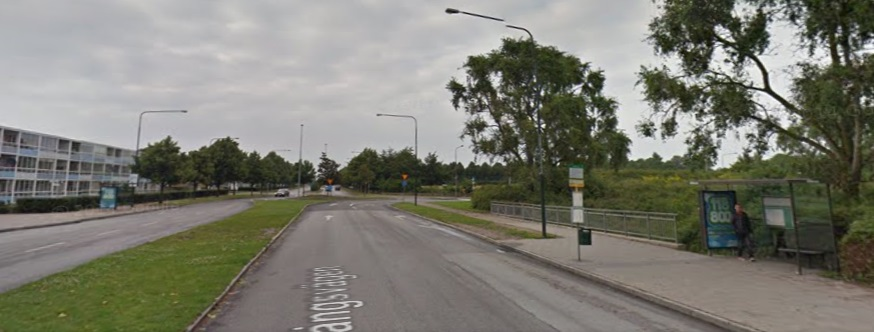
\includegraphics[width=\linewidth]{lind.jpg}
  \caption{En obevakad hållplats i Malmös stadsdel Lindängen. (Google Maps: Lindängen - Malmö)}
  \label{fig:lind}
\end{figure}




% ---------------------------------------------------------------------------
%: ----------------------- end of thesis sub-document ------------------------
% ---------------------------------------------------------------------------

